\documentclass[twoside]{book}

% Packages required by doxygen
\usepackage{fixltx2e}
\usepackage{calc}
\usepackage{doxygen}
\usepackage[export]{adjustbox} % also loads graphicx
\usepackage{graphicx}
\usepackage[utf8]{inputenc}
\usepackage{makeidx}
\usepackage{multicol}
\usepackage{multirow}
\PassOptionsToPackage{warn}{textcomp}
\usepackage{textcomp}
\usepackage[nointegrals]{wasysym}
\usepackage[table]{xcolor}

% Font selection
\usepackage[T1]{fontenc}
\usepackage[scaled=.90]{helvet}
\usepackage{courier}
\usepackage{amssymb}
\usepackage{sectsty}
\renewcommand{\familydefault}{\sfdefault}
\allsectionsfont{%
  \fontseries{bc}\selectfont%
  \color{darkgray}%
}
\renewcommand{\DoxyLabelFont}{%
  \fontseries{bc}\selectfont%
  \color{darkgray}%
}
\newcommand{\+}{\discretionary{\mbox{\scriptsize$\hookleftarrow$}}{}{}}

% Page & text layout
\usepackage{geometry}
\geometry{%
  a4paper,%
  top=2.5cm,%
  bottom=2.5cm,%
  left=2.5cm,%
  right=2.5cm%
}
\tolerance=750
\hfuzz=15pt
\hbadness=750
\setlength{\emergencystretch}{15pt}
\setlength{\parindent}{0cm}
\setlength{\parskip}{3ex plus 2ex minus 2ex}
\makeatletter
\renewcommand{\paragraph}{%
  \@startsection{paragraph}{4}{0ex}{-1.0ex}{1.0ex}{%
    \normalfont\normalsize\bfseries\SS@parafont%
  }%
}
\renewcommand{\subparagraph}{%
  \@startsection{subparagraph}{5}{0ex}{-1.0ex}{1.0ex}{%
    \normalfont\normalsize\bfseries\SS@subparafont%
  }%
}
\makeatother

% Headers & footers
\usepackage{fancyhdr}
\pagestyle{fancyplain}
\fancyhead[LE]{\fancyplain{}{\bfseries\thepage}}
\fancyhead[CE]{\fancyplain{}{}}
\fancyhead[RE]{\fancyplain{}{\bfseries\leftmark}}
\fancyhead[LO]{\fancyplain{}{\bfseries\rightmark}}
\fancyhead[CO]{\fancyplain{}{}}
\fancyhead[RO]{\fancyplain{}{\bfseries\thepage}}
\fancyfoot[LE]{\fancyplain{}{}}
\fancyfoot[CE]{\fancyplain{}{}}
\fancyfoot[RE]{\fancyplain{}{\bfseries\scriptsize Generated by Doxygen }}
\fancyfoot[LO]{\fancyplain{}{\bfseries\scriptsize Generated by Doxygen }}
\fancyfoot[CO]{\fancyplain{}{}}
\fancyfoot[RO]{\fancyplain{}{}}
\renewcommand{\footrulewidth}{0.4pt}
\renewcommand{\chaptermark}[1]{%
  \markboth{#1}{}%
}
\renewcommand{\sectionmark}[1]{%
  \markright{\thesection\ #1}%
}

% Indices & bibliography
\usepackage{natbib}
\usepackage[titles]{tocloft}
\setcounter{tocdepth}{3}
\setcounter{secnumdepth}{5}
\makeindex

% Hyperlinks (required, but should be loaded last)
\usepackage{ifpdf}
\ifpdf
  \usepackage[pdftex,pagebackref=true]{hyperref}
\else
  \usepackage[ps2pdf,pagebackref=true]{hyperref}
\fi
\hypersetup{%
  colorlinks=true,%
  linkcolor=blue,%
  citecolor=blue,%
  unicode%
}

% Custom commands
\newcommand{\clearemptydoublepage}{%
  \newpage{\pagestyle{empty}\cleardoublepage}%
}

\usepackage{caption}
\captionsetup{labelsep=space,justification=centering,font={bf},singlelinecheck=off,skip=4pt,position=top}

%===== C O N T E N T S =====

\begin{document}

% Titlepage & ToC
\hypersetup{pageanchor=false,
             bookmarksnumbered=true,
             pdfencoding=unicode
            }
\pagenumbering{alph}
\begin{titlepage}
\vspace*{7cm}
\begin{center}%
{\Large S\+Q\+U\+A\+RE }\\
\vspace*{1cm}
{\large Generated by Doxygen 1.8.13}\\
\end{center}
\end{titlepage}
\clearemptydoublepage
\pagenumbering{roman}
\tableofcontents
\clearemptydoublepage
\pagenumbering{arabic}
\hypersetup{pageanchor=true}

%--- Begin generated contents ---
\chapter{Решатель квадратных ур-\/ний V0.0.0-\/000}
\label{index}\hypertarget{index}{}~\newline
\begin{DoxyAuthor}{Author}
Титов ЕМ ~\newline
Файлы\+: ~\newline

\begin{DoxyItemize}
\item \hyperlink{main_8cpp}{main.\+cpp}
\item \hyperlink{_square_res_8cpp}{Square\+Res.\+cpp} 
\end{DoxyItemize}
\end{DoxyAuthor}

\chapter{R\+E\+A\+D\+ME}
\label{md__r_e_a_d_m_e}
\Hypertarget{md__r_e_a_d_m_e}
S\+Q\+U\+A\+RE -\/ Решатель квадратных уравнений 
\chapter{File Index}
\section{File List}
Here is a list of all files with brief descriptions\+:\begin{DoxyCompactList}
\item\contentsline{section}{\hyperlink{main_8cpp}{main.\+cpp} }{\pageref{main_8cpp}}{}
\item\contentsline{section}{\hyperlink{_square_res_8cpp}{Square\+Res.\+cpp} }{\pageref{_square_res_8cpp}}{}
\end{DoxyCompactList}

\chapter{File Documentation}
\hypertarget{main_8cpp}{}\section{main.\+cpp File Reference}
\label{main_8cpp}\index{main.\+cpp@{main.\+cpp}}
{\ttfamily \#include $<$stdio.\+h$>$}\newline
{\ttfamily \#include \char`\"{}Square\+Res.\+cpp\char`\"{}}\newline
Include dependency graph for main.\+cpp\+:
\nopagebreak
\begin{figure}[H]
\begin{center}
\leavevmode
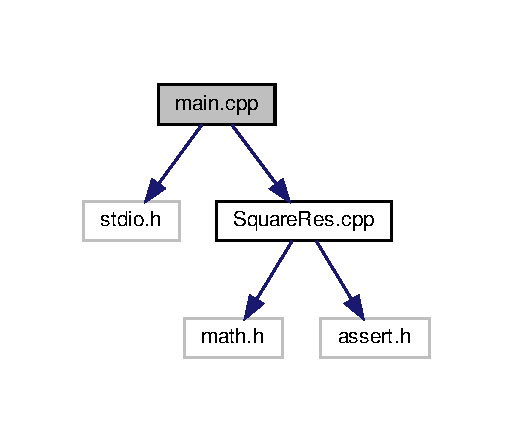
\includegraphics[width=246pt]{main_8cpp__incl}
\end{center}
\end{figure}
\subsection*{Functions}
\begin{DoxyCompactItemize}
\item 
int \hyperlink{main_8cpp_a539716722220e7fb08fbce2070b75adf}{User\+Fr\+Read} (unsigned int Num\+Elem, long double $\ast$Elements, const char $\ast$Greeting, int Max\+Tries)
\item 
int \hyperlink{main_8cpp_af9a3c657f416e33c6c94ff0936df9b63}{Fill} (long double $\ast$mas, unsigned int N\+UM, long double filler)
\item 
int \hyperlink{main_8cpp_ae66f6b31b5ad750f1fe042a706a4e3d4}{main} ()
\end{DoxyCompactItemize}
\subsection*{Variables}
\begin{DoxyCompactItemize}
\item 
const int \hyperlink{main_8cpp_a58732d68137f37824a99677c89169763}{M\+A\+X\+T\+R\+I\+ES} = 3
\begin{DoxyCompactList}\small\item\em Макс. кол-\/во попыток ввода \end{DoxyCompactList}\end{DoxyCompactItemize}


\subsection{Function Documentation}
\mbox{\Hypertarget{main_8cpp_af9a3c657f416e33c6c94ff0936df9b63}\label{main_8cpp_af9a3c657f416e33c6c94ff0936df9b63}} 
\index{main.\+cpp@{main.\+cpp}!Fill@{Fill}}
\index{Fill@{Fill}!main.\+cpp@{main.\+cpp}}
\subsubsection{\texorpdfstring{Fill()}{Fill()}}
{\footnotesize\ttfamily int Fill (\begin{DoxyParamCaption}\item[{long double $\ast$}]{mas,  }\item[{unsigned int}]{N\+UM,  }\item[{long double}]{filler }\end{DoxyParamCaption})}

Заполняет(инициализирует) массив указанными числами 
\begin{DoxyParams}[1]{Parameters}
\mbox{\tt in}  & {\em mas} & (long double$\ast$) указатель на массив \\
\hline
\mbox{\tt in}  & {\em N\+UM} & (unsigned int) число элементов массива \\
\hline
\mbox{\tt in}  & {\em filler} & (long double) число для заполнения\\
\hline
\end{DoxyParams}


Definition at line 87 of file main.\+cpp.

\mbox{\Hypertarget{main_8cpp_ae66f6b31b5ad750f1fe042a706a4e3d4}\label{main_8cpp_ae66f6b31b5ad750f1fe042a706a4e3d4}} 
\index{main.\+cpp@{main.\+cpp}!main@{main}}
\index{main@{main}!main.\+cpp@{main.\+cpp}}
\subsubsection{\texorpdfstring{main()}{main()}}
{\footnotesize\ttfamily int main (\begin{DoxyParamCaption}{ }\end{DoxyParamCaption})}

\begin{DoxyReturn}{Returns}
Номер ошибки ~\newline
1 -\/ ошибка выполнения \hyperlink{_square_res_8cpp_a701a0c4aee5f746c18eb110e1d5a8261}{Square\+Res()} ~\newline
2 -\/ ошибка ввода
\end{DoxyReturn}


Definition at line 20 of file main.\+cpp.

\mbox{\Hypertarget{main_8cpp_a539716722220e7fb08fbce2070b75adf}\label{main_8cpp_a539716722220e7fb08fbce2070b75adf}} 
\index{main.\+cpp@{main.\+cpp}!User\+Fr\+Read@{User\+Fr\+Read}}
\index{User\+Fr\+Read@{User\+Fr\+Read}!main.\+cpp@{main.\+cpp}}
\subsubsection{\texorpdfstring{User\+Fr\+Read()}{UserFrRead()}}
{\footnotesize\ttfamily int User\+Fr\+Read (\begin{DoxyParamCaption}\item[{unsigned int}]{Num\+Elem,  }\item[{long double $\ast$}]{Elements,  }\item[{const char $\ast$}]{Greeting,  }\item[{int}]{Max\+Tries }\end{DoxyParamCaption})}

Считывает числа в массив 
\begin{DoxyParams}[1]{Parameters}
\mbox{\tt in}  & {\em Num\+Elem} & (unsigned int) число элементов массива \\
\hline
\mbox{\tt in}  & {\em Elements} & (long double$\ast$) указатель на массив \\
\hline
\mbox{\tt in}  & {\em Greeting} & (const char$\ast$) Приветствие на ввод \\
\hline
\mbox{\tt in}  & {\em Max\+Tries} & (int) Макимальное кол-\/во попыток ввода элемента \\
\hline
\end{DoxyParams}
\begin{DoxyReturn}{Returns}
0 -\/ считывание успешно; 1 -\/ превышено макс кол-\/во попыток ввода
\end{DoxyReturn}


Definition at line 52 of file main.\+cpp.



\subsection{Variable Documentation}
\mbox{\Hypertarget{main_8cpp_a58732d68137f37824a99677c89169763}\label{main_8cpp_a58732d68137f37824a99677c89169763}} 
\index{main.\+cpp@{main.\+cpp}!M\+A\+X\+T\+R\+I\+ES@{M\+A\+X\+T\+R\+I\+ES}}
\index{M\+A\+X\+T\+R\+I\+ES@{M\+A\+X\+T\+R\+I\+ES}!main.\+cpp@{main.\+cpp}}
\subsubsection{\texorpdfstring{M\+A\+X\+T\+R\+I\+ES}{MAXTRIES}}
{\footnotesize\ttfamily const int M\+A\+X\+T\+R\+I\+ES = 3}



Макс. кол-\/во попыток ввода 



Definition at line 18 of file main.\+cpp.


\hypertarget{_r_e_a_d_m_e_8md}{}\section{R\+E\+A\+D\+M\+E.\+md File Reference}
\label{_r_e_a_d_m_e_8md}\index{R\+E\+A\+D\+M\+E.\+md@{R\+E\+A\+D\+M\+E.\+md}}

\hypertarget{_square_res_8cpp}{}\section{Square\+Res.\+cpp File Reference}
\label{_square_res_8cpp}\index{Square\+Res.\+cpp@{Square\+Res.\+cpp}}
{\ttfamily \#include $<$math.\+h$>$}\newline
{\ttfamily \#include $<$assert.\+h$>$}\newline
Include dependency graph for Square\+Res.\+cpp\+:
\nopagebreak
\begin{figure}[H]
\begin{center}
\leavevmode
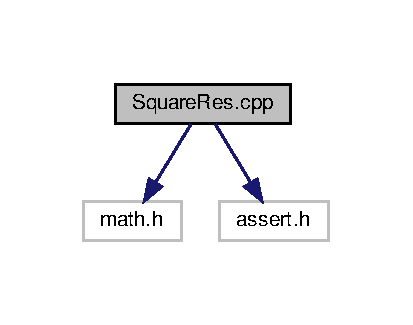
\includegraphics[width=198pt]{_square_res_8cpp__incl}
\end{center}
\end{figure}
This graph shows which files directly or indirectly include this file\+:
\nopagebreak
\begin{figure}[H]
\begin{center}
\leavevmode
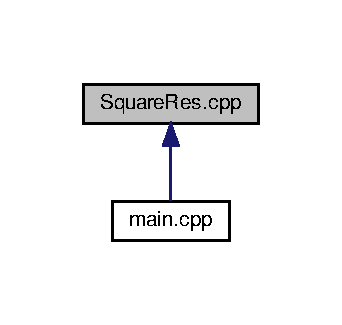
\includegraphics[width=164pt]{_square_res_8cpp__dep__incl}
\end{center}
\end{figure}
\subsection*{Macros}
\begin{DoxyCompactItemize}
\item 
\#define \hyperlink{_square_res_8cpp_a423e5a7bfec38724690b61f5a7fed838}{I\+N\+F\+IN}~-\/1
\begin{DoxyCompactList}\small\item\em Константа обозначает бескнечное кол-\/во корней \end{DoxyCompactList}\item 
\#define \hyperlink{_square_res_8cpp_a9c7b069fee3c8184e14a7de8e5da2dc6}{P\+R\+E\+C\+I\+S\+I\+ON}~32
\begin{DoxyCompactList}\small\item\em Константа указывает точность сранение чисел с плавабщей точкой (кол-\/во знаков после запятой) \end{DoxyCompactList}\end{DoxyCompactItemize}
\subsection*{Functions}
\begin{DoxyCompactItemize}
\item 
int \hyperlink{_square_res_8cpp_aab842cd94b3bf15e007dc497f0a31d08}{fl\+C\+O\+MP} (long double t1, long double t2, int precision)
\item 
void \hyperlink{_square_res_8cpp_a952ecdf4c8265b10b53138cc9b295e13}{Linear\+Res} (long double a, long double b, long double $\ast$x)
\item 
int \hyperlink{_square_res_8cpp_a701a0c4aee5f746c18eb110e1d5a8261}{Square\+Res} (long double a, long double b, long double c, long double $\ast$x1, long double $\ast$x2)
\end{DoxyCompactItemize}


\subsection{Macro Definition Documentation}
\mbox{\Hypertarget{_square_res_8cpp_a423e5a7bfec38724690b61f5a7fed838}\label{_square_res_8cpp_a423e5a7bfec38724690b61f5a7fed838}} 
\index{Square\+Res.\+cpp@{Square\+Res.\+cpp}!I\+N\+F\+IN@{I\+N\+F\+IN}}
\index{I\+N\+F\+IN@{I\+N\+F\+IN}!Square\+Res.\+cpp@{Square\+Res.\+cpp}}
\subsubsection{\texorpdfstring{I\+N\+F\+IN}{INFIN}}
{\footnotesize\ttfamily \#define I\+N\+F\+IN~-\/1}



Константа обозначает бескнечное кол-\/во корней 



Definition at line 5 of file Square\+Res.\+cpp.

\mbox{\Hypertarget{_square_res_8cpp_a9c7b069fee3c8184e14a7de8e5da2dc6}\label{_square_res_8cpp_a9c7b069fee3c8184e14a7de8e5da2dc6}} 
\index{Square\+Res.\+cpp@{Square\+Res.\+cpp}!P\+R\+E\+C\+I\+S\+I\+ON@{P\+R\+E\+C\+I\+S\+I\+ON}}
\index{P\+R\+E\+C\+I\+S\+I\+ON@{P\+R\+E\+C\+I\+S\+I\+ON}!Square\+Res.\+cpp@{Square\+Res.\+cpp}}
\subsubsection{\texorpdfstring{P\+R\+E\+C\+I\+S\+I\+ON}{PRECISION}}
{\footnotesize\ttfamily \#define P\+R\+E\+C\+I\+S\+I\+ON~32}



Константа указывает точность сранение чисел с плавабщей точкой (кол-\/во знаков после запятой) 



Definition at line 8 of file Square\+Res.\+cpp.



\subsection{Function Documentation}
\mbox{\Hypertarget{_square_res_8cpp_aab842cd94b3bf15e007dc497f0a31d08}\label{_square_res_8cpp_aab842cd94b3bf15e007dc497f0a31d08}} 
\index{Square\+Res.\+cpp@{Square\+Res.\+cpp}!fl\+C\+O\+MP@{fl\+C\+O\+MP}}
\index{fl\+C\+O\+MP@{fl\+C\+O\+MP}!Square\+Res.\+cpp@{Square\+Res.\+cpp}}
\subsubsection{\texorpdfstring{fl\+C\+O\+M\+P()}{flCOMP()}}
{\footnotesize\ttfamily int fl\+C\+O\+MP (\begin{DoxyParamCaption}\item[{long double}]{t1,  }\item[{long double}]{t2,  }\item[{int}]{precision }\end{DoxyParamCaption})}

Сравнивает 2 числа с точностью до precision знаков после запятой 
\begin{DoxyParams}[1]{Parameters}
\mbox{\tt in}  & {\em t1} & (long double) 1е число \\
\hline
\mbox{\tt in}  & {\em t2} & (long double) 2е число \\
\hline
\mbox{\tt in}  & {\em precision} & (int) точность \\
\hline
\end{DoxyParams}
\begin{DoxyReturn}{Returns}
1 Если t1$>$t2; -\/1 Если t2$>$t1; 0 если t1=t2
\end{DoxyReturn}


Definition at line 49 of file Square\+Res.\+cpp.

\mbox{\Hypertarget{_square_res_8cpp_a952ecdf4c8265b10b53138cc9b295e13}\label{_square_res_8cpp_a952ecdf4c8265b10b53138cc9b295e13}} 
\index{Square\+Res.\+cpp@{Square\+Res.\+cpp}!Linear\+Res@{Linear\+Res}}
\index{Linear\+Res@{Linear\+Res}!Square\+Res.\+cpp@{Square\+Res.\+cpp}}
\subsubsection{\texorpdfstring{Linear\+Res()}{LinearRes()}}
{\footnotesize\ttfamily void Linear\+Res (\begin{DoxyParamCaption}\item[{long double}]{a,  }\item[{long double}]{b,  }\item[{long double $\ast$}]{x }\end{DoxyParamCaption})}

Решает линейное уравнение 
\begin{DoxyParams}[1]{Parameters}
\mbox{\tt in}  & {\em a} & (long double) коэф-\/т при 1й степени \\
\hline
\mbox{\tt in}  & {\em b} & (long double) коэф-\/т при 0й степени \\
\hline
\mbox{\tt in}  & {\em x} & (long double$\ast$) указатель на корень\\
\hline
\end{DoxyParams}


Definition at line 65 of file Square\+Res.\+cpp.

\mbox{\Hypertarget{_square_res_8cpp_a701a0c4aee5f746c18eb110e1d5a8261}\label{_square_res_8cpp_a701a0c4aee5f746c18eb110e1d5a8261}} 
\index{Square\+Res.\+cpp@{Square\+Res.\+cpp}!Square\+Res@{Square\+Res}}
\index{Square\+Res@{Square\+Res}!Square\+Res.\+cpp@{Square\+Res.\+cpp}}
\subsubsection{\texorpdfstring{Square\+Res()}{SquareRes()}}
{\footnotesize\ttfamily int Square\+Res (\begin{DoxyParamCaption}\item[{long double}]{a,  }\item[{long double}]{b,  }\item[{long double}]{c,  }\item[{long double $\ast$}]{x1,  }\item[{long double $\ast$}]{x2 }\end{DoxyParamCaption})}

Записывает корни по адресам $\ast$x1 $\ast$x2 
\begin{DoxyParams}[1]{Parameters}
\mbox{\tt in}  & {\em a} & (long double) 1й коэф-\/т \\
\hline
\mbox{\tt in}  & {\em b} & (long double) 2й коэф-\/т \\
\hline
\mbox{\tt in}  & {\em c} & (long double) 3й коэф-\/т \\
\hline
\mbox{\tt in}  & {\em x1} & ($\ast$long double) указатель на 1й корень \\
\hline
\mbox{\tt in}  & {\em x2} & ($\ast$long double) указатель на 2й корень \\
\hline
\end{DoxyParams}
\begin{DoxyReturn}{Returns}
Количество корней (0, 1, 2) или I\+N\+F\+IN -\/ бесконечное кол-\/во решений
\end{DoxyReturn}


Definition at line 13 of file Square\+Res.\+cpp.


%--- End generated contents ---

% Index
\backmatter
\newpage
\phantomsection
\clearemptydoublepage
\addcontentsline{toc}{chapter}{Index}
\printindex

\end{document}
